%!TEX root = ../../main.tex


\begin{figure}[!htb]
\centering
%\hrulefill \\
%\vspace{5pt}
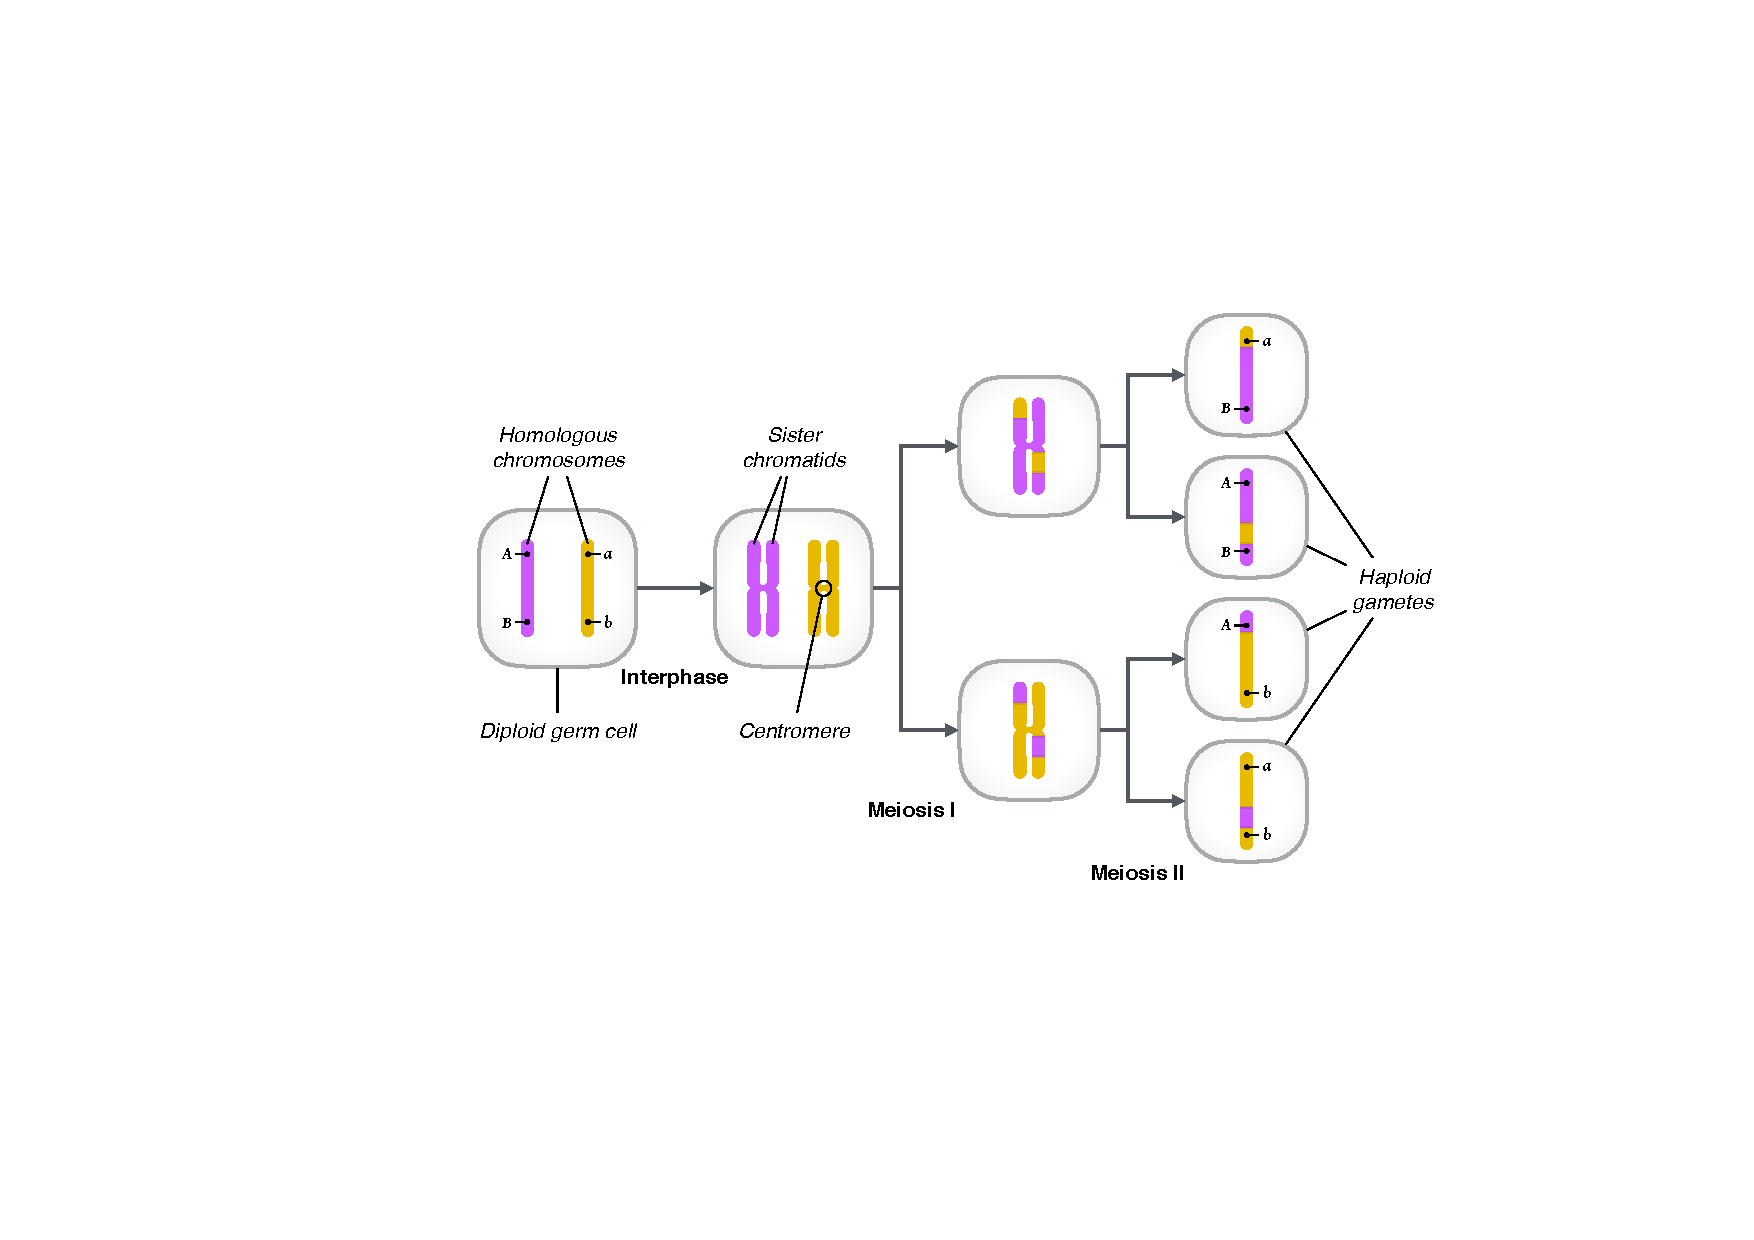
\includegraphics[width=\textwidth]{./img/ch1/info_meiosis}
\Caption{Illustration of recombination during meiosis}
{\N{1} pair of homologous chromosomes is shown at the beginning of the meiotic cell cycle (\emph{left}).
Maternal and paternal chromosomes are shown in \emph{purple} and \emph{yellow} (arbitrarily coloured).
The allelic configuration at \n{2} sites is indicated on both chromosomes; $(A,B)$ and $(a,b)$.
\Gls{dna} sequences are replicated during the \emph{Interphase} of meiosis, where each chromosome forms \n{2} identical \emph{sister chromatids} which are held together at the \emph{centromere}.
Homologous chromosomes are paired at the beginning of the first cell division (\emph{Meiosis~I}), during which sequence segments are exchanged between chromatids through crossover.
In the second cell division (\emph{Meiosis~II}), the \n{4} chromatids are then separated into haploid gametes (\emph{right}).}
{fig:info_meiosis}
% \vspace{-5pt}
% \hrulefill%
\end{figure}
